\documentclass[12pt,fleqn]{jarticle}


\usepackage{amsmath,amssymb}
\usepackage[dvipdfmx]{graphicx}
\usepackage{subfigure}
\usepackage{epsfig}

\renewcommand{\figurename}{Fig.}
\setlength{\baselineskip}{12pt}
\topmargin -0.5cm
\textheight 24cm
\textwidth 15cm
\oddsidemargin 1cm
%
\newcommand{\sgn}{\mathop{\rm sgn}}
\newcommand{\sat}{\mathop{\rm sat}}
\newcommand{\bx}{\mbox{\boldmath$x$}}
\newcommand{\T}{\mathsf{T}}
\newcommand{\dd}{\text{d}}
%
\date{}
%
\begin{document}

\thispagestyle{empty}
\vspace{5em}
{\Large


\vspace{5em}

\begin{center}
\vspace*{25.4truemm}
\centerline{\LARGE \bf 2025年度}
\vskip 2pc
\centerline{\Huge \bf メカニカルデザインコース}
\vskip 2pc
\centerline{\Huge \bf レポート}
\vskip 3pc
\centerline{\LARGE \bf 準\ \ \ 備\ \ \ 資\ \ \ 料}
\vskip 3pc
\centerline{\Large \bf 学籍番号:20******}
\vskip 3pc
\centerline{\Large \bf 氏名:名無権平}
\vskip 10pc

%\small{\tt http://www.me.saga-u.ac.jp/$\sim$sato}\\
\vspace{1em}
%\small{\tt sato@me.saga-u.ac.jp}
\end{center}
}
\vspace{2em}


\clearpage
\clearpage
%
\newpage

%%%%%%%%%%%%%%%%%%%%%%%%%%%%%%%%%%%%%%%%%%%%%%%%%%


%%%%%%%%%%%%%%%%%%%%%%%%%%%%%%%%%%%%%%%%%%%%%%%%%%
\section{式や図の記述方法}
\subsection{式の記述例}
\begin{equation}
    \left\{
    \begin{aligned}
    u(t) =& \; k_c \left(k_1(t) e(t) + \int_0^t k_2(t) e(\tau) d\tau \right) \\
    {k}_1(t) =& \; k_p(t) + \alpha_1 k_i(t) \\
    {k}_2(t) =& \; \alpha_2 k_i(t)\\
    k_p(t) =& \; e^2(t), 
    \dot k_i(t) = \; e^2(t)
    \end{aligned}
    \right.
    \label{eq:PI}
\end{equation}

ここで, $\alpha_1$ と $\alpha_2$ はある正定数である.\\
(\ref{eq:PI})式は, Pゲインを${k_1}(t)$で, Iゲインを${k_2}(t)$で調整する一種の適応的パラメータ調整則を持つPI制御法である.
$\alpha_1$ と $\alpha_2$ は, 設計パラメータとして選ぶことができる.
%%%%%%%%%%%%%%%%%%%%%%%%%%%%%%%%%%%%%%%%%%%%%%%%%%
\subsection{図の表示例1}
\begin{figure}[h]
    \centering
    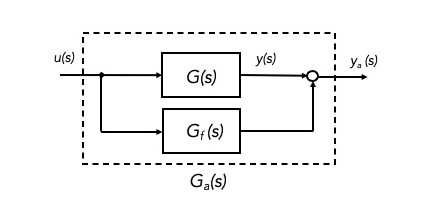
\includegraphics[scale=0.7]{./fig/PFC.jpg}
    \caption{図の表示}
    \label{fig:sample_1}
\end{figure}

%%%%%%%%%%%%%%%%%%%%%%%%%%%%%%%%%%%%%%%%%%%%%%%%%%
\clearpage
%%%%%%%%%%%%%%%%%%%%%%%%%%%%%%%%%%%%%%%%%%%%%%%%%%
\subsection{図の表示例2}

\begin{figure}[h]
    \centering
    \subfigure[例1]{
     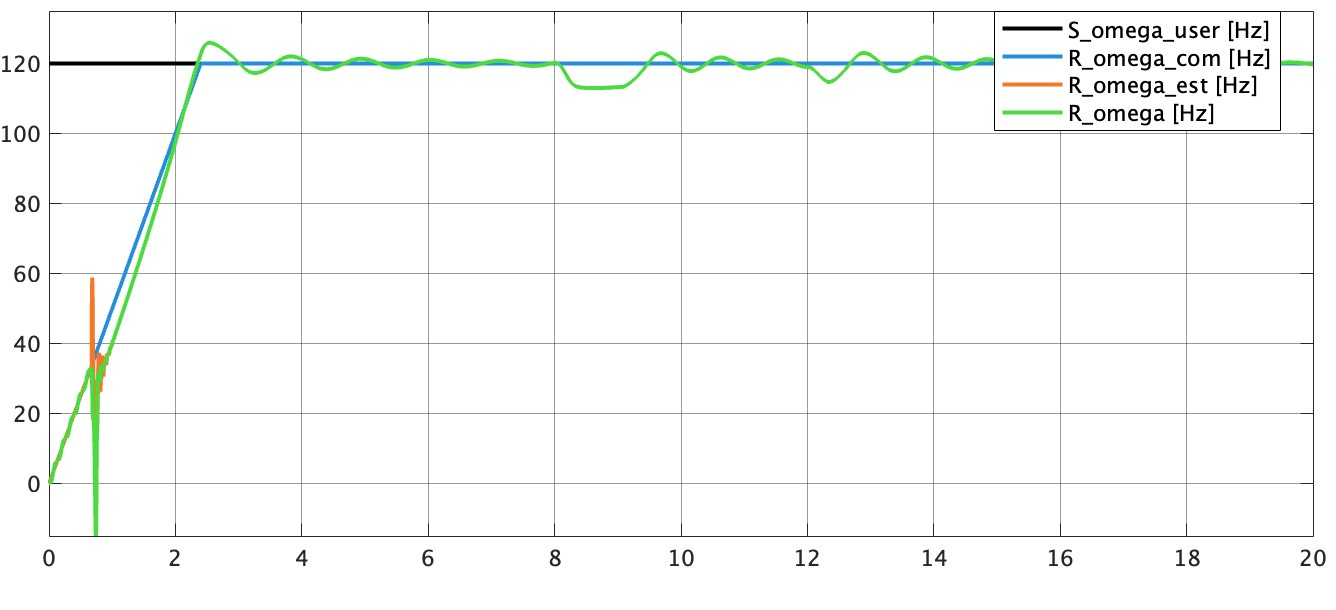
\includegraphics[scale=0.1]{./fig/pfc_none_output.jpg}
    }
    \subfigure[例2]{
    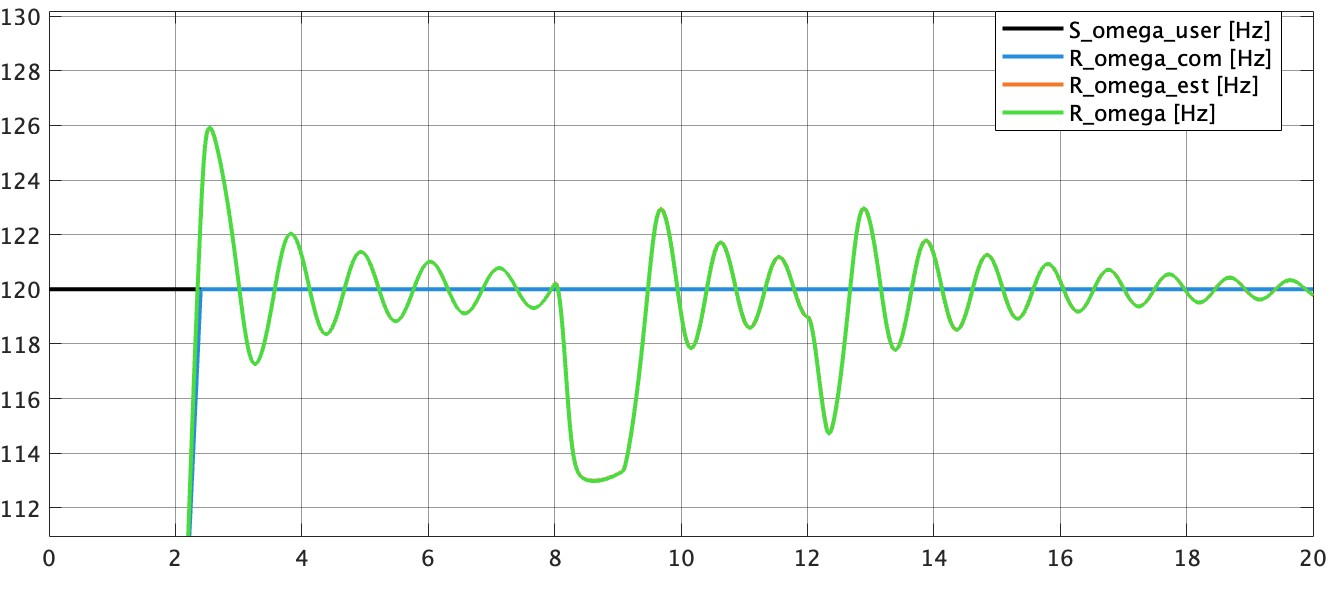
\includegraphics[scale=0.1]{./fig/pfc_none_output_range.jpg}
    }
    \caption{横並びでも図の表示できるよ}
    \label{fig:sample_2}
\end{figure}
%%%%%%%%%%%%%%%%%%%%%%%%%%%%%%%%%%%%%%%%%%%%%%%%%%

\end{document}
